\chapter{Utilizzo di OpenStack}\label{sec:openstack_usage}

All'interno di questo capitolo verranno spiegati tutti i concetti base che servono per un primo utilizzo di OpenStack. Verranno anche date le istruzioni per eseguire le operazioni principali, come ad esempio creare una rete o una macchina virtuale, in modo che anche chi non ha mai utilizzato questa piattaforma possa orientarsi e farsi un'idea generale sulle funzionalità che offre.

\section{Identity}

\subsection{Domains}

Un dominio di OpenStack è un contenitore ad alto livello per progetti, gruppi e utenti. Ciascun dominio definito all'interno di un cloud OpenStack è completamente indipendente dagli altri; questo permette di avere entità (per esempio utenti, gruppi o progetti) con gli stessi nomi definiti in domini diversi. Inoltre gli utenti di domini diversi possono essere rappresentati da diversi backend di autenticazione e avere attributi diversi ma devono obbligatoriamente essere mappati sugli stessi set di ruoli e privilegi che sono stati utilizzati per definire le policy di sicurezza in modo da poter avere accesso ai servizi del cloud.

Per creare un dominio è necessario accedere con un utente amministratore. Una volta eseguito il login si deve aprire il menu a tendina denominato \textit{Identity} e selezionare la voce \textit{Domains}. A questo punto verrà visualizzata la pagina con tutti i domini presenti all'interno del cloud e per crearne uno nuovo sarà sufficiente cliccare sul pulsante \textit{Create Domain} e inserire i dati richiesti. Se si vogliono aggiungere entità al dominio appena creato (per esempio utenti, progetti, ecc.) sarà necessario cliccare sul pulsante \textit{Set Domain Context} accanto al nome del dominio; in questo modo il context della sessione verrà cambiato in modo da attivare il dominio selezionato e poter modificare le sua entità.

\subsection{Groups}

I gruppi di OpenStack sono dei contenitori ai quali appartengono degli utenti. Possono essere utilizzati per garantire l'accesso a progetti o semplicemente per raggruppare gli utenti.

Per creare un gruppo è necessario accedere all'interfaccia con un utente amministratore o con privilegi di amministrazione all'interno del dominio. Una volta eseguito l'accesso si deve aprire il menu a tendina \textit{Identity} e selezionare la voce \textit{Groups}. Cliccando sul pulsante \textit{Create Group} verrà visualizzato un form tramite il quale sarà possibile creare il nuovo gruppo.

\subsection{Roles}

I ruoli sono delle entità associate agli utenti e, dato che OpenStack usa un approccio RBAS (Role-Based Access Control), servono per determinare quali azioni ciascun utente può compiere. 

\subsection{Projects}

Un progetto è un contenitore di entità (utenti, istanze, ecc.) che a sua volta fa parte di un dominio. A differenza di un dominio il progetto possiede alcune entità univoche e altre che possono essere in comune con altri progetti; per esempio un'istanza può far parte solamente di un progetto, mentre un utente può far parte di più progetti.

Per creare un progetto è necessario eseguire l'accesso all'interfaccia con un utente amministratore o con privilegi di amministrazione all'interno del dominio. Una volta eseguito l'accesso si deve aprire il menu a tendina \textit{Identity} e selezionare la voce \textit{Projects}. Cliccando poi sul pulsante \textit{Create Project} verrà aperto un form composto da tre schede:
\begin{itemize}
    \item \textbf{Project Information}: permette di specificare le informazioni generiche del progetto (nome, descrizione, ecc.)
    \item \textbf{Project Members}: permette di selezionare gli utenti che hanno accesso al progetto
    \item \textbf{Project Groups}: permette di selezionare i gruppi che fanno parte del progetto
\end{itemize}

\noindent
Se si utilizza Horizon (l'interfaccia Web di OpenStack) è possibile accedere solamente ad un progetto per volta, ovvero visualizzare le entità del progetto selezionato. Per cambiare la selezione del progetto è necessario cliccare sul nome del progetto attualmente selezionato nella barra di navigazione in cima alla pagine (come mostrato in \cref{fig:openstack_project_selection}) e successivamente selezionare dal menu a tendina il progetto che si vuole utilizzare.

\begin{figure}[H]
    \center
    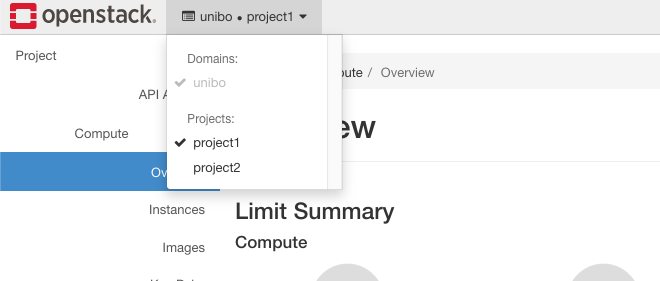
\includegraphics[width=0.9\linewidth]{tesi/files/immagini/openstack_usage/openstack_project_switch.png}
    \caption{Selezione del progetto tramite l'interfaccia Web.}
    \label{fig:openstack_project_selection}
\end{figure}

\subsection{Users}

Gli user, come ci su può aspettare, sono gli utenti che utilizzano il cloud OpenStack. Ciascun utente può essere membro di uno o più progetti, di uno o più gruppi e può avere uno o più ruoli. È possibile autenticare gli utenti in modi differenti utilizzando provider di autenticazione esterni (per esempio LDAP, SSO, ecc.); nel caso di questo progetto è stato utilizzato il provider di default di OpenStack.

Per creare un utente è necessario eseguire l'accesso all'interfaccia con un utente amministratore o con privilegi di amministrazione all'interno del dominio. Una volta eseguito l'accesso si deve aprire il menu a tendina \textit{Identity} e selezionare la voce \textit{Users}. In questo modo verrà aperta la pagine contenente tutti gli utenti del dominio che si sta visualizzando e, cliccando sul pulsante \textit{Crete User} in alto a destra, sarà possibile crearne uno nuovo. È possibile inserire numerose informazioni riguardanti ciascun utente ma quelle fondamentali sono Username, Password e Primary Project; se non viene scelto nessun progetto verrà negato l'accesso al nuovo utente nonostante sia abilitato.

\section{Network}

\subsection{Networks e Subnets}

Una network in OpenStack è una rete virtuale che sta alla base della comunicazione tra macchine virtuali, container o altri dispositivi virtuali che comunicano tramite rete.
% 
Ciascuna network può contenere al suo interno una o più subnet che hanno la stessa funzionalità delle VLAN in una rete fisica: 
% 
servono per suddividere logicamente la rete in più sezioni separate, ciascuna delle quali possiede un proprio range di indirizzi IP ed è indipendente dalle altre.

Per creare una rete è necessario aprire il menu a tendina \textit{Project} > \textit{Network} e selezionare la voce \textit{Networks}; questo aprirà la pagina dove vengono visualizzate tutte le reti. A questo punto, cliccando sul pulsante \textit{Create Network}, verrà visualizzato il form per creare la nuova rete. Spuntato la casella \textit{Enable Admin State} la rete verrà automaticamente abilitata dopo la creazione e, spuntando \textit{Create Subnet}, viene data anche la possibilità di creare direttamente una subnet. Tramite il parametro \textit{MTU} è possibile anche configurare la dimensione massima che possono avere i pacchetti che vengono inviati sulla rete.

Con un utente con privilegi di amministrazione è possibile anche creare una rete pubblica, ovvero una rete che possiede una subnet con indirizzi IP pubblici a cui tutti gli utenti possono collegarsi, in modo che gli host della rete possano essere raggiunti direttamente dall'esterno.

Per creare una subnet invece è necessario andare alla pagine dove vengono visualizzate tutte le reti e cliccare sul nome di quella che si vuole utilizzare; questo aprirà la pagina di dettaglio della rete. Una volte fatto questo si deve passare alla scheda denominata \textit{Subnets} e cliccare sul pulsante \textit{Subnets}; a questo punto verrà visualizzato un form suddiviso in due schede dove andranno inserite tutte le informazioni riguardanti la nuova subnet che si vuole creare. I campi richiesti sono i seguenti:
\begin{itemize}
    \item \textbf{Subnet Name}: nome della subnet (arbitrario)
    \item \textbf{Network Address}: spazio degli indirizzi IP (in formato CIDR) che appartengono alla subnet (per esempio \texttt{10.0.0.0/24})
    \item \textbf{IP Version}: versione del protocollo IP
    \item \textbf{Gateway IP}: indirizzo IP del gateway; se non si desidera aggiungere un gateway alla subnet è possibile spuntare la casella \texttt{Disable Gateway} per disabilitarlo
    \item \textbf{Enable DHCP}: se spuntato, il server DHCP viene abilitato per la nuova subnet
    \item \textbf{Allocation Polls}: permette di indicare i range di indirizzi IP che possono essere assegnati dinamicamente; si deve inserire un pool per ciascuna riga nel formato \texttt{start\_ip,end\_ip} (per es. \texttt{10.0.0.128,10.0.0.253})
    \item \textbf{DNS Name Servers}: permette di specificare i server DNS per la subnet (uno per riga)
    \item \textbf{Host Routes}: permette di specificare delle regole di routing statiche che verranno applicate agli host; ciascuna entry deve essere nel formato \texttt{destination\_cidr,nexthop} (per es. \texttt{192.168.1.0/24,10.0.0.1})
\end{itemize}

\subsection{Routers}

Un router virtuale OpenStack ha esattamente le stesse funzioni di un router fisico in una rete fisica: permette agli host della rete di raggiungere subnet diverse dalla propria. Il router supporta sia il routing statico sia diversi protocolli di routing dinamico, come ad esempio OSPF e BGP. Ciascun router può avere una o più interfacce virtuali che possono essere collegate a diverse subnet appartenenti alla stessa rete o a reti diverse. I router possono avere un numero indefinito di interffacce di rete virtuali e quindi possono essere collegati a tutte le subnet desiderate; inoltre, se una delle interfacce viene collegata ad una rete pubblica, permettono a ciascuno degli host presenti sulle subnet private di accedere a internet utilizzando la tecnica del NAT.

Per creare un router è necessario aprire il menu a tendine \textit{Project} > \textit{Network} e selezionare la voce \textit{Routers}; in questa pagina verranno mostrati tutti i router appartenenti al progetto corrente. Cliccando sul pulsante \textit{Create Router} verrà mostrato il form che permette di creare il nuovo router con i seguenti campi che, oltre a campi simili a quelli visti in precedenza, contiene il campo \emph{External Network} che permette di specificare una rete esterna a cui collegare il router. Questo campo non è obbligatorio ma se si desidera far accedere gli host delle subnet collegate al router a internet senza un indirizzo IP pubblico è necessario impostarlo.
% 
Dopo aver creato il router è possibile aggiungere le interfacce virtuali che lo collegano alle subnet; per fare questo si deve cliccare sul nome del router in modo da aprire la pagina con tutte le informazioni, aprire la scheda \textit{Iterfaces} e cliccare sul pulsante \textit{Add Interface}. A questo punto comparirà un form che permette di selezionare quale subnet collegare al router e opzionalmente l'indirizzo IP da assegnargli all'interno della subnet selezionata.

Nel caso in cui il router sia stato collegato ad una rete esterna, nella pagina di dettaglio con tutte le informazioni riguardanti il router è possibile visualizzare il suo indirizzo IP pubblico nella sezione \emph{External Gateway}. Questo permette di verificare se il router funziona semplicemente facendo un ping all'indirizzo mostrato.

\begin{figure}[ht]
   \center
   % 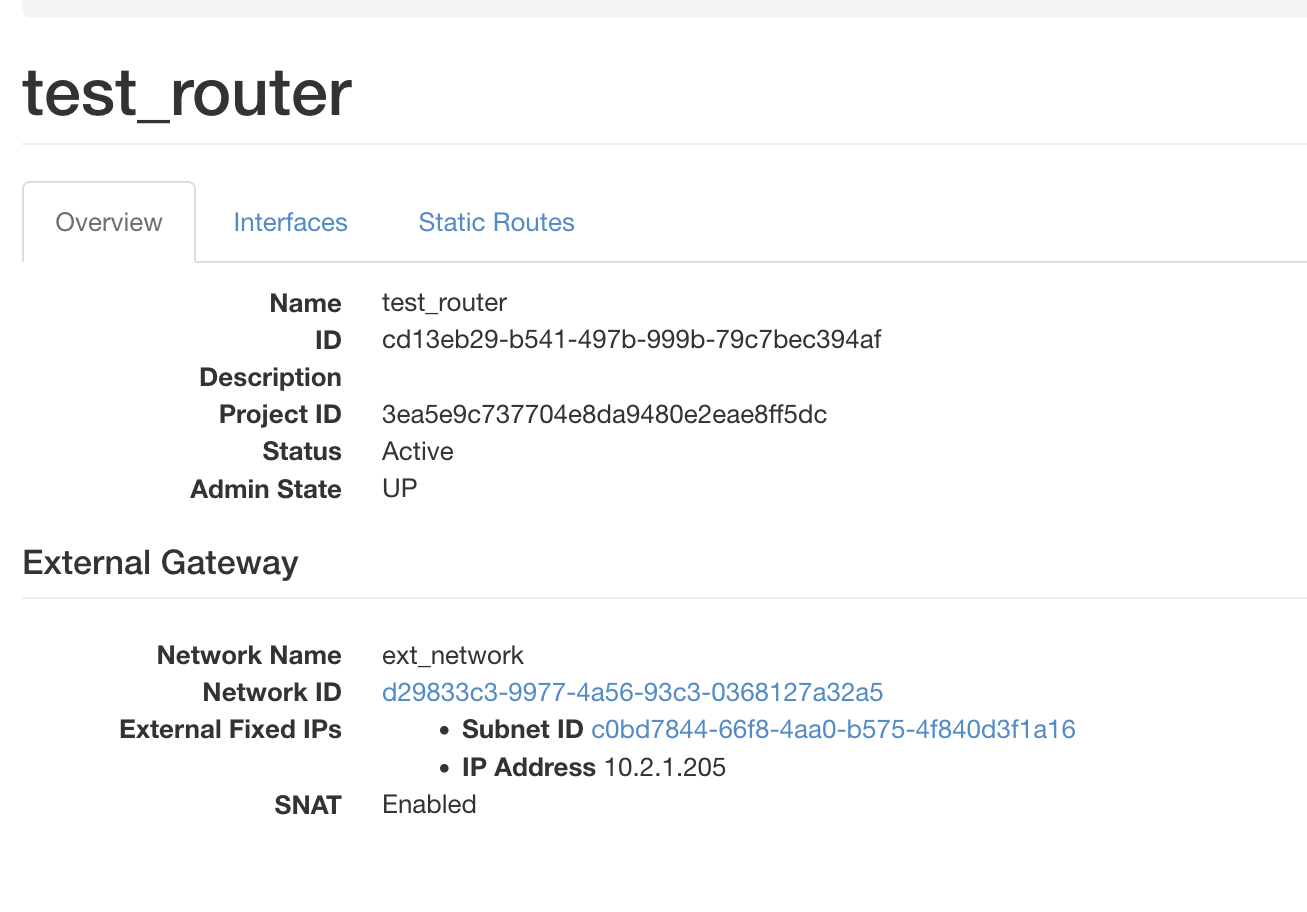
\includegraphics[scale=0.4]{tesi/files/immagini/openstack_usage/openstack_router_info.png}
   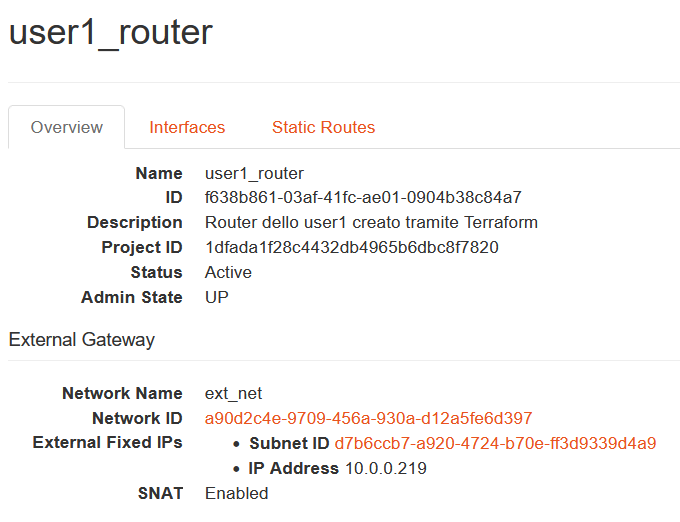
\includegraphics[width=0.9\linewidth]{tesi/files/immagini/openstack_usage/openstack_router_info_2.png}
   \caption{Pagina con le informazioni di un router.}
   \label{fig:openstack_router_info}
\end{figure}

\subsection{Security Groups}

I \textit{Security Groups} sono l'equivalente dei firewall virtuali che controllano il traffico in entrata e in uscita per ciascun host. Permettono di specificare regole secondo diversi criteri come ad esempio gli indirizzi IP della sorgente e del destinatario o le porte. Ciascun \textit{Security Group} può avere un numero indefinito di regole e può essere assegnato a più di un host; ogni host può avere a sua volta più di un \textit{Security Group}.

Per creare un \textit{Security Group} da interfaccia grafica è necessario aprire il menu a tendina \textit{Project} > \textit{Network} e cliccare sulla voce \textit{Security Groups}; in questo modo verrà aperta la pagina che mostra tutti i gruppi presenti all'interno del progetto corrente. Cliccando sul pulsante \textit{Create Security Group} in alto a destra verrà aperto un form che permetterà di specificare nome e descrizione del nuovo gruppo. Per modificare le regole del \textit{Security Group} appena creato si deve cliccare il pulsante \textit{Manage Rules} sulla stessa riga del nome; a questo punto verrà caricata una pagina con la lista delle regole già presenti; per crearne una nuova è necessario cliccare sul pulsante \textit{Add Rule} che farà comparire un form con i seguenti campi:
\begin{itemize}
    \item \textbf{Rule}: permette di selezionare il protocollo che si vuole filtrare; sono già presenti numerosi protocolli standard (per esempio HTTP, HTTPS, SSH, ecc.) ma viene anche data la possibilità di definire regole personalizzate sia su protocollo TCP che su UDP
    \item \textbf{Direction}: permette di specificare se la regola deve essere applicata al traffico in entrata (Ingress) o in uscita (Egress)
    \item \textbf{Open Port}: permette di decidere se la regole deve essere applicata ad una sola porta, ad un range di porte o a tutte le porte per il protocollo selezionato
    \item \textbf{Port}: viene visualizzato solo se la regola viene applicata ad una sola porta e permette di specificare la suddetta porta
    \item \textbf{From Port} e \textbf{To Port}: vengono visualizzati solo se la regola viene applicata ad un range di porte e permettono di specificare rispettivamente la porta iniziale e quella finale
    \item \textbf{Remote}: permette di specificare che la regola deve filtrare per \emph{CIDR} o \emph{Security group}; nel primo caso verranno fatti passare i pacchetti che provengono da un indirizzo appartenente alla subnet definita mentre nel secondo caso verranno fatti passare solo i pacchetti che provengono da un host che possiede un \textit{Security Group} definito
    \item \textbf{CIDR}: viene visualizzato solo se il campo \emph{Remote} è impostato su \emph{CIDR}; permette di impostare il range di indirizzi IP da filtrare in formato \emph{CIDR}
    \item \textbf{Security Group} e \textbf{Ether Type}: vengono visualizzati solo se il campo \emph{Remote} è impostato su \emph{Security Group}; permettono di specificare rispettivamente il \emph{Security Group} a cui è consentito l'accesso e la versione del protocollo IP
\end{itemize}

\subsection{Floating IPs}

I \textit{Floating IPs} sono indirizzi IP pubblici che possono essere assegnati ad un host connesso ad una rete privata e che gli permettono di essere raggiunto anche dall'esterno. Ciascun IP può essere assegnato e rilasciato in qualsiasi momento e addirittura può essere assegnato a host differenti in momenti diversi.

Per ottenere un \textit{Floating IP} da associare ad un host è necessario aprire il menu a tendina \textit{Project} > \textit{Network} e selezionare la voce \textit{Floating IPs}. In questa pagina verranno visualizzati tutti gli indirizzi IP ottenuti per il progetto corrente. Per allocarne uno nuovo è necessario cliccare sul pulsante \textit{Allocate IP To Project}; a questo punto comparirà il form di allocazione che permette di scegliere, tra le altre cose, il pool di indirizzi pubblici da cui prelevare il nuovo IP.

Per assegnare un \textit{Floating IP} ad un'istanza è necessario accedere alla pagina con la lista delle istanza aprendo il menu a tendina \textit{Project} > \textit{Compute} e selezionare la voce \textit{Instances}. A questo punto si deve individuare l'istanza nella tabella e poi cliccare il pulsante \textit{Associate Floating IP} nella colonna \emph{Action}; in questo modo verrà visualizzato il form che permetterà di associare all'istanza un Floating IP esistente oppure di allocarne uno nuovo e poi assegnarlo.



\section{Storage}

\subsection{Volumes}

Un volume è un disco virtuale che può essere collegato ad un'istanza e su cui vengono salvati i dati. Ha esattamente la stessa funzione di un HDD o SSD all'interno di un computer fisico. I volumi possono essere creati al momento della creazione dell'istanza oppure tramite l'apposita pagina all'interno dell'interfaccia web.

Per crearne uno è necessario aprire il menu a tendina \textit{Project} > \textit{Volumes} e selezionare la voce \textit{Volumes}; qui verranno visualizzati tutti i volumi appartenenti al progetto corrente. Cliccando sul pulsante \textit{Create Volume} verrà mostrato il form che permette di creare un nuovo volume specificandone tutti i parametri compresa la dimensione massima.

\subsection{Snapshots}

Gli snapshot sono come delle fotografie dei volumi. Permettono di eseguire un'istantanea del volume in un qualsiasi momento e di salvarla in modo che in caso di problemi, come ad esempio un cancellazione involontaria di dati, si possa ripristinare il sistema esattamente com'era. Vengono spesso usati per creare backup o per clonare un sistema con lo scopo di eseguire test o di modificarlo.

\section{Compute}

\subsection{Flavors}\label{sec:flavor}

I \textit{Flavors} sono configurazioni predefinite per le risorse da assegnare ad una istanza; al loro interno contengono il numero di CPU, la quantità di RAM e lo spazio di storage predefinito da assegnare ad un'istanza quando viene creata. I \textit{Flavors} hanno il compito di creare dei modelli di istanze tra cui i client possono scegliere in base alle risorse di cui hanno bisogno e, all'interno dei cloud provider pubblici come ad esempio AWS, hanno anche lo scopo di definire il costo di una determinata istanza.

Per creare un \textit{Flavor} è necessario eseguire il login con un utente con privilegi di amministrazione; una volta fatto questo si deve aprire il menu a tendina \textit{Admin} > \textit{Compute} e selezionare la voce \textit{Flavors}. A questo punto si aprirà la pagina contente tutti i \textit{Flavors} definiti all'interno del cloud; per crearne uno nuovo si deve cliccare il pulsante \emph{Create Flavor} e compilare il form composto dai seguenti campi:
\begin{itemize}
    \item \textbf{Name}: nome del flavor
    \item \textbf{ID}: id del flavor; inserendo la stringa \emph{auto} viene generato in automatico
    \item \textbf{VCPUs}: numero di CPU virtuali a disposizione dell'istanza
    \item \textbf{RAM (MB)}: quantità in MB di RAM a disposizione dell'istanza
    \item \textbf{Root Disk (GB)}: dimensione in GB del volume principale
    \item \textbf{Ephemeral Disk (GB)}: dimensione in GB dello storage temporaneo non persistente dell'istanza
    \item \textbf{Swap Disk (MB)}: dimensione in MB della memoria swap
    \item \textbf{RX/TX Factor}: indica la larghezza di banda in percentuale che l'istanza può utilizzare; i valori devono essere espressi in un numero decimale tra 0 e 1
\end{itemize}
È possibile inoltre restringere l'accesso al \textit{Flavor} a specifici progetti tramite la scheda \emph{Flavor Access} presente nel form.


\subsection{Key Pairs}
Le coppie di chiavi (\textit{Key Pairs}) sono coppie composte da una chiave privata ed una pubblica che servono per accedere alle istanze create tramite il protocollo SSH. È possibile sia importare una chiave pubblica precedentemente generata sia creare la coppia di chiavi direttamente dall'interfaccia web. Nel secondo caso la chiave pubblica verrà memorizzata sul cloud mentre quella privata verrà scaricata in automatico e immediatamente eliminata.

Per gestire le coppie di chiavi pubbliche è necessario aprire il menu a tendina \textit{Project} > \textit{Compute} e selezionare la voce \textit{Key Pairs}. A questo punto per creare una nuova coppia di chiavi si deve cliccare sul pulsante \textit{Create Key Pair}, mentre per importare una chiave pubblica già esistente si deve cliccare su \textit{Import Public Key}.

Per gestire le coppie di chiavi è necessario aprire il menu a tendina \textit{Project} > \textit{Compute} e selezionare la voce \textit{Key Pairs}. A questo punto per creare una nuova coppia di chiavi si deve cliccare sul bottone \textit{Create Key Pair}, mentre per importare una chiave pubblic già esistente si deve cliccare su \textit{Import Public Key}.

\subsection{Images}
Le immagini sono template di macchine virtuali preconfigurate che fungono da base per la creazione di nuove istanze. Solitamente un'immagine è composta solamente dal sistema operativo di base configurato in modo da importare in automatico una chiave pubblica per consentire l'accesso alla nuova istanza tramite SSH senza l'utilizzo di password. Questo permette agli utilizzatori del cloud di avere piena autonomia nella costruzione delle loro istanze e quindi dell'infrastruttura che desiderano.

Per creare una nuova immagine da interfaccia grafica si deve aprire il menu a tendina \textit{Project} > \textit{Compute} e selezionare la voce \textit{Images}. A questo punto cliccando sul pulsante \textit{Create Image} verrà visualizzato il form che permette la creazione dell'immagine e che contiene i seguenti campi:
\begin{itemize}
    \item \textbf{Image Name}: nome della nuova immagine
    \item \textbf{Image Description}: descrizione della nuova immagine
    \item \textbf{File}: file da caricare con l'immagine
    \item \textbf{Format}: formato dell'immagine
    \item \textbf{Architecture}: architettura del sistema operativo all'interno dell'immagine
    \item \textbf{Minimum Disk (GB)}: dimensione minima in GB del volume di storage
    \item \textbf{Minimum RAM (MB)}: dimensione minima in MB della memoria RAM
    \item \textbf{Visibility}: visibilità della nuova immagine agli altri utenti del cloud
    \item \textbf{Protected}: permette di proteggere l'immagine da cancellazioni accidentali
\end{itemize}

\subsection{Instances}\label{sec:openstack_usage_instances}

Un'istanza è una vera e propria macchina virtuale che viene istanziata partendo da un'immagine. 

Per creare una nuova istanza è necessario aprire il menu a tendina a sinistra \textit{Project} > \textit{Compute}, selezionare la voce \textit{Instances} e, una volta caricata la pagina con le informazioni su tutte le istanze del progetto, cliccare sul pulsante \textit{Launch Instance}. In questo modo si aprirà un form con diverse schede da compilare con tutti i dati della nuova istanza; ciascuna di queste schede verrà trattata nei paragrafi seguenti.

\paragraph{Details.}

\begin{itemize}
    \item \textbf{Project Name}: nome del progetto; non è possibile selezionare un progetto diverso da quello attivo nella sessione, quindi se si vuole cambiare si deve fare prima della creazione dell'istanza
    \item \textbf{Instance Name}: nome dell'istanza
    \item \textbf{Description}: descrizione dell'istanza
    \item \textbf{Availability Zone}: nel caso in cui siano configurate più availability zones questo parametro permette di scegliere in quale di queste creare l'istanza
    \item \textbf{Count}: indica il numero di istanze da creare con la configurazione che si sta specificando
\end{itemize}

\paragraph{Source.}
\begin{itemize}
    \item \textbf{Select Boot Source}: permette di selezionare la sorgente dalla quale creare l'istanza; tale sorgente può essere un'immagine, un volume già esistente o uno snapshot
    \item \textbf{Create New Volume}: permette di specificare se creare un nuovo volume per l'istanza o se utilizzare un disco temporaneo; nel caso in cui si scelga come boot source un volume esistente questo parametro non viene mostrato
    \item \textbf{Volume Size}: permette di specificare la dimensione del nuovo volume (nel caso in cui venga creato)
    \item \textbf{Delete Volume on Instance Delete}: permette di specificare se il volume associato all'istanza (nel caso in cui esista) deve essere cancellato contemporaneamente all'istanza o meno
    \item \textbf{Allocated}: permette di selezionare la sorgente da cui viene creata la nuova istanza
\end{itemize}

\paragraph{Flavor.}
Questa scheda permette semplicemente di scegliere il flavor (ovvero la quantità di risorse) da assegnare alla nuova istanza

\paragraph{Networks.}
Questa scheda permettere di scegliere a quali reti collegare la nuova istanza; è possibile collegare un numero indefinito di reti alle istanze.

\paragraph{Security Groups.}
In questa scheda è possibile scegliere i security groups da associare alla nuova istanza.

\paragraph{Key Pair.}
Questa scheda permette di selezionare la chiave pubblica da importare all'interno dell'istanza in modo da poter eseguire l'accesso tramite SSH utilizzando la relativa chiave privata.

\paragraph{Configuration.}
All'interno di questa scheda è possibile inserire uno script che verrà eseguito all'avvio della macchina e che permette di configurare l'istanza in modo totalmente automatico. Permette inoltre di eseguire il partizionamento manuale del volume nel caso in cui ne sia stato aggiunto uno.
